\documentclass{article}

\usepackage{amsmath,amsfonts,amsthm,amssymb}
\usepackage{fancyhdr}
\usepackage{lastpage}
\usepackage{graphicx}
\usepackage{supertabular}
\usepackage{multirow}
\usepackage{ifthen}
\usepackage{enumerate}

% In case you need to adjust margins:
\topmargin=-0.5in
\evensidemargin=0in
\oddsidemargin=0in
\textwidth=6.5in
\textheight=9.0in
\headsep=0.25in

% Homework Specific Information
\newcommand{\hmwkTitle}{Project Report 2}
\newcommand{\hmwkDueDate}{March 17th, 2014}
\newcommand{\hmwkClass}{42-731}
\newcommand{\hmwkSection}{A}
\newcommand{\hmwkAuthor}{Alex Sun Yoo, Michael Nye, Ozan Iskilibli}
\newcommand{\hmwkEmail}{ayoo, mnye, oiskilib}
\newcommand{\hmwkCollaborators}{}
\newcommand{\bigspace}{\vspace{.25in}}

% Tools for formatting questions
\newcommand{\question}[1] {\vspace{.25in} \hrule\vspace{0.5em}
\noindent{\bf #1} \vspace{0.5em}
\hrule \vspace{.10in}}
\renewcommand{\part}[1] {\vspace{.10in} {\bf (#1)}}

% Setup the header and footer
\pagestyle{fancyplain}
\lhead{\fancyplain{}{\hmwkAuthor \\ \hmwkEmail}}
\chead{\fancyplain{}{\textbf{\hmwkTitle}}}
\rhead{\fancyplain{}{\hmwkClass\hmwkSection \\ Due:\ \hmwkDueDate} }
\lfoot{}
\cfoot{}
\rfoot{Page\ \thepage\ of\ \pageref{LastPage}}
\renewcommand\headrulewidth{0.4pt}
\renewcommand\footrulewidth{0.4pt}

% Format paragraphs to have spacing instead of indents
\setlength{\parindent}{0pt}
\setlength{\parskip}{5pt plus 1pt}

% This is used to trace down (pin point) problems
% in latexing a document:
%\tracingall

\renewcommand{\arraystretch}{1.5}

%%%%%%%%%%%%%%%%%%%%%%%%%%%%%%%%%%%%%%%%%%%%%%%%%%%%%%%%%%%%%

\begin{document}

\thispagestyle{plain}
\begin{center}
{\Large \hmwkClass\ \hmwkTitle} \\
\hmwkAuthor \\
\hmwkEmail \\
\ifthenelse{\equal{\hmwkCollaborators}{}}{}{Collaborators: \hmwkCollaborators\\}
\ifthenelse{\equal{\hmwkSection}{}}{}{Section \hmwkSection\\}
Due: \hmwkDueDate\\
\end{center}
%%%%%%%%%%%%%%%%%%%%%%%%%%%%%%%%%%%%%%%%%%%%%%%%%%%%%%%%%%%%%

\question{Part 1: Particle Feature Detection}

\textbf{B.2.1}

\textbf{B.2.2}

Using a 5x5 mask detects noticeably fewer local extrema than using a 3x3 mask, as shown in Figures ~\ref{fig:extrema_3}
and ~\ref{fig:extrema_5}. This is because with a larger mask, the tested point is compared with a larger area of neighboring
points, reducings its chances of being classified as a local extrema.

\begin{figure}[h]
\centering
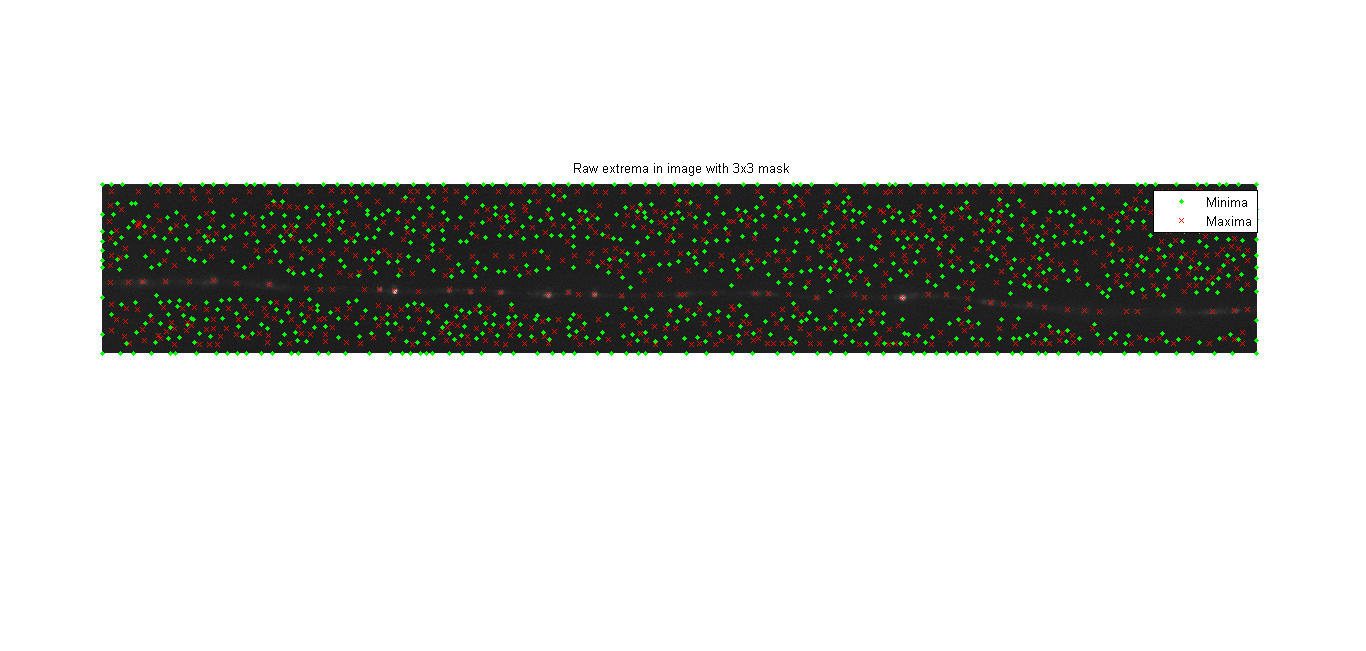
\includegraphics[width=12cm]{extrema_mask_3.png}
\caption{Local Extrema (3x3 mask)}
\label{fig:extrema_3}
\end{figure}

\begin{figure}[h]
\centering
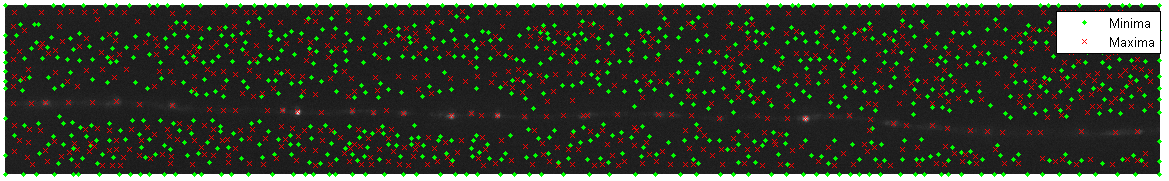
\includegraphics[width=12cm]{extrema_mask_5.png}
\caption{Local Extrema (5x5 mask)}
\label{fig:extrema_5}
\end{figure}



\textbf{B.2.3}


\textbf{B.2.4}




\pagebreak
\question{Part 2: Sub-pixel Resolution Particle Detection}



\textbf{B.3.1}


\textbf{B.3.2}




%%%%%%%%%%%%%%%%%%%%%%%%%%%%%%%%%%%%%%%%%%%%%%%%%%%%%%%%%%%%%

\end{document}

%%%%%%%%%%%%%%%%%%%%%%%%%%%%%%%%%%%%%%%%%%%%%%%%%%%%%%%%%%%%%
